Graph embeddings is about finding different representations of graphs. For example, we can find an embedding of nodes to $d$-dimensions so that similar nodes have embeddings that are close together. 

\subsection{Linear node embeddings}
    The only thing we are going to assume for linear node embeddings is that we have a graph $G$ with $V$ as the vertex set and $A$ as the (assumed to be binary) adjacency matrix. 
    
    We can use the similarity between two nodes as our embedding function. For example, say we have $similarity(u,v) \approx z_v^T z_u$, then the similarity is our map to the embedding space. If two elements are similar, they should land close to each other in the embedding space. 
    
    In order to learn node embeddings, we need to define an \emph{encoder} which is a mapping from nodes to embeddings. We also need to define a \emph{node similarity function}, which is a measure of similarity in the original network, and finally optimize the parameters of the encoder such that 
    \m{
        Similarity(u, v) \approx z_v^T z_u
    }
    The encoder maps each node to a low dimensional vector $ENC(V) = z_v$. The similarity function specifies how relationships in vector space maps to relationships in the original network. What the similarity function means, is that the similarity in the original network should be approx the similarity of the node embeddings.
    
\subsubsection{Shallow encoding}
    \textbf{Shallow} encoding is the most simple form of embedding. Here the encoder is a simple lookup. $ENC(v) = Zv$ where $Z \in \R^{d \times |V|}$ where each column is a node embedding (what we learn). $v \in \I^{|V|}$ is an indicator with all zeroes except a one in the column indicating node $v$. Each node is assigned a unique embedding vector. 
    
\subsubsection{Similarity}
    The key distinction between shallow methods is how they define similarity. When should two nodes be similar? 
    \begin{itemize}
        \item If they are connected?
        \item If they share neighbours?
        \item Have similar structural roles?
        \item Semantically similar?
        \item Etc?
    \end{itemize}
    
\subsubsection{Adjacency-based similarity}
    With \textbf{adjacency-based similarity}, our similarity is the edge weight between nodes. Our intuition is that dot products between embeddings should approximate edge existence. Our loss is then
    
    \m{
        L = \sum_{(u, v) \in V \times V} |z_u^T z_v - A_{uv}|^2
    }
    We then need to find an embedding matrix $Z \in \R^{d \times |V|}$ that minimizes the loss $L$. We can use the effective stochastic gradient descent, we can also use a matrix decomposition solver, which works in limited cases. 
    The drawbacks of adjacency-based similarity is that it takes $O(|V|^2)$ time because we have to consider all node pairs. We also have $O(|V|)$ parameters. It also onlu considers direct, local connections. 
    
\subsubsection{Multi-hop similarity}
    With multi-hop similarity, we consider $k$-hop neighbours. It basically means the set of nodes that is reachable from the origin within $k$ hops. 
    
    The idea is to use the loss function
    \m{
        L = \sum_{(u,v) \in V \times V}{|| z_u^T z_v - A_{u,v}^k||^2}
    }
    Note the $A^k$ part. We train embeddings to predict $k$-hop neighbours. In practice (GraRep from Cao et al), use log-transformed probabilistic adjacency matrix
    \m{
        \tilde{A}_{i,j}^k = \max(
            \log(\frac{A_{i,h / d_i}}{\sum_{l \in V}(A_{l, j}/d_l)^k})^k - \alpha, 0
        )
    }
    $d$ is node degree, and $\alpha$ is a constant shift. We train multiple different hop lengths and concat the output. 
    
    Another option in multi-hop similarity is to measure the overlap between node neighbourhoods, using overlap functions such as Jaccard similarity and Adamic-Adar score which is $A(u, v) = \sum_{i \in N(u) \cap N(v)} \frac{1}{\log||N(i)}$. Our loss function is then
    
    \m{\sum_{(u,v) \in V \times V}||z_u^T z_v - S_{u,v}||^2}
    
    So far all we have done is to define pairwise similarities and then optimize low dimensional embeddings to approximate these pairwise similarities. The issues is that these are generally expensive $O(|V|^2)$, since we need to iterate over all pairs of nodes. They are also brittle, because we must hand design deterministic similarity measures. $O(|V|)$ is also a massive parameter space.
    
\subsection{Neural Embeddings}
    \subsubsection{Random walk similarity}
    Another way to define similarity is to use the ability to walk between vertices. Here we can define $z_u^T z_v$ as the probability that $u$ and $v$ co-occur in a random walk over our over network. 
    
    Specifically, we can estimate the probability of visiting node $v$ starting from $u$ using some random walk strategy, then we can optimize embeddings to encode these random walk statistics. 
    
    A benefit to using random walks is \emph{expressivity}. There is a flexible stochastic definition of node similarity that incorporates both local and global neighborhood information. Another is \emph{efficiency}. We do not need to consider all node pairs when training. 
    
    The strategy for optimization is as follows
    \begin{enumerate}
        \item Run short random walks starting from each node using strategy $R$
        \item For each node $u$, collect $N_R(u)$, the multiset of nodes visited on random walks starting from $u$
        \item We then optimize embeddings according to \m{
            L = \sum_{u \in V} \sum_{v \in N_R(u)} - log(p(v | z_u))}
    \end{enumerate}
    
    Our intuition here is to optimize embeddings to maximize the likelihood of random walk co-occurrences. We can parameterize $p(v | z_u)$ using softmax \m{
        p(v | z_u) = \frac{\exp(z_u^T z_v)}{\sum_{n \in V} \exp(z_u^T z_n)}
    }

    Let us put things together. We get a loss function of \m{
        L = \sum_{u \in V} \sum_{v \in N_R(u)} - \log(\frac{\exp(z_u^T z_v)}{\sum_{n \in V}{\exp(z_u^T z_n)}})
    }
    Here the double sum is the sum for all nodes of all nodes seen on the random walk, then in the log we have the predicted probability of $u$ and $v$ co-occurring on random walk. 

    A problem with this approach, is that the nested sums give $O(|V|^2)$. The bottom part of the fraction (the normalization term) is bad, but can we approximate it? 
    
    We can use negative sampling. Our log term is approx
    \m{
        \log(\sigma(z_u^T z_v)) - \sum_{i=1}^{k}\log(\sigma(z_u^T z_{ni}))
    }
    Where $n_i \sim p_V$, $\sigma$ is the sigmoid function and $p_V$ is a random distribution over all the nodes. We sample the negative nodes proportional to degree. The more we sample, the more robust our estimates. A higher $k$ corresponds to higher prior on negative events. 
    
\subsection{General similarities}
    The characteristics of RW approaches is
    \begin{itemize}
        \item Similarity is fixed to random walks
        \item Expressive and non-linear
        \item Can scale up with sampling techniques
    \end{itemize}
    The characteristics of matrix factorization approaches
    \begin{itemize}
        \item Similarity can be flexible
        \item Constrained to linear models (such as SVD)
        \item Scales if the matrix is sparse
    \end{itemize}
    
    If we consider linear models, they are linear and interactions are local. However, if we recall PPR. \m{
        PPR(V) = (I - \alpha A \Delta^{-1})^{-1}(1- \alpha)v
    }
    Where $v$ is the indicator vector for $v$. We can factorize PPR of a graph with generalized SVD. It scales extremely well, but it is linear. Say we have $S_v$ which is the PPR starting from node $v$. If we compute these using different restart vectors. \m{
        S_u = cMS_u + (1-c)p_u
    }
    then we can run the algorithm to find the PPR once for each node and put is intro matrix S. These will be probability distributions. The matrix is then $S \in \R^{n \times n}$.
    
    How do we get the embeddings from this similarity matrix?? We can learn the distribution of nodes using a non-linear method, or use SVD on the similarity matrix. 
    
    Let us first recap SVD. Any $n \times m$ matrix $A$ can be factored into
    \m{
        A = U \Sigma V^T
    }
    Where $U \in \R^{n \times K}, V \in \R^{m \times K}$ where $K = \min(m, n)$. $\Sigma$ is a diagonal matrix with elements $\sigma_1 \geq \dots \geq \sigma_K$. If $rank(A) = r$, then $\sigma_{r+1} = \dots = \sigma_k = 0$.
    
    The \textbf{Eckart-Young theorem} says that the best low-rank approximation can be computed by SVD. 
    
    The second approach is \texbf{VERSE}. We can compute an embedding $Z$ that preserves the similarities expressed as a distribution over the nodes. 
    
    We can use KL-divergence between the distribution of node $p$ and node $q$. \m{
        D(p || q) = \sum_{x}p(x) \log(\frac{p(x)}{q(x)})
    }
    This can also be written as $-p(x) \log q(x)$.
    
    We will use a one-layer neural network parameterized by $n \times d$ matrix $Z$. 
    
    The similarity of one to all is then (we use softmax normalization) \m{
        sim(v, \cdot) = \frac{e^{z_v z^T}}{\sum_{i=1}^{n} e^{z_v z_i}}
    }
    Our total loss is then
    \m{
        L = - \sum_{v \in V} s_v \log sim(v, \cdot)
    }
    
    This can be sped up with Noise Contrastive Estimation.
    
\subsubsection{Random walk approaches: DeepWalk}
    First we need to mention that the volume of a graph $vol(G) = \sum_{i} \sum_j A_{i,j}$. One random walk approach is DeepWalk. It goes as follows:
    \begin{enumerate}
        \item For $n = 1, 2, \dots, N$
        \item Pick $w_i^n$ according to probability distribution $P(w_1)$
        \item Generate vertex sequence $(w_^n, \dots, w_L^n)$ of length $L$ by random walk on network $G$
        \item \begin{enumerate}
            \item For $j = 1, 2, \dots, L - T$ 
            \item add vertex-context pair $(w_j^n, w_{j+r}^n)$ to multiset $D$
            \item add vertex-context pair $(w_{j+r}^n, w_j^n)$ to multiset $D$
        \end{enumerate}
    \end{enumerate}
    Run SGNS on $d$ with $k$ negative samples \footnote{Elaborate on SGNS}
    
\subsection{Graph neural networks}
    Say we have a graph $G$ with matrix of node features $X \in R^{m \times |V|}$, which could be labels, attributes etc. 
    
\subsubsection{Neighborhood aggregation}
    
    Our idea is to generate node embeddings based on local neighborhoods. We call this neighborhood aggregation. Our intuition is that nodes should aggregate information from their neighbors using neural networks. 
    
    \begin{center}
        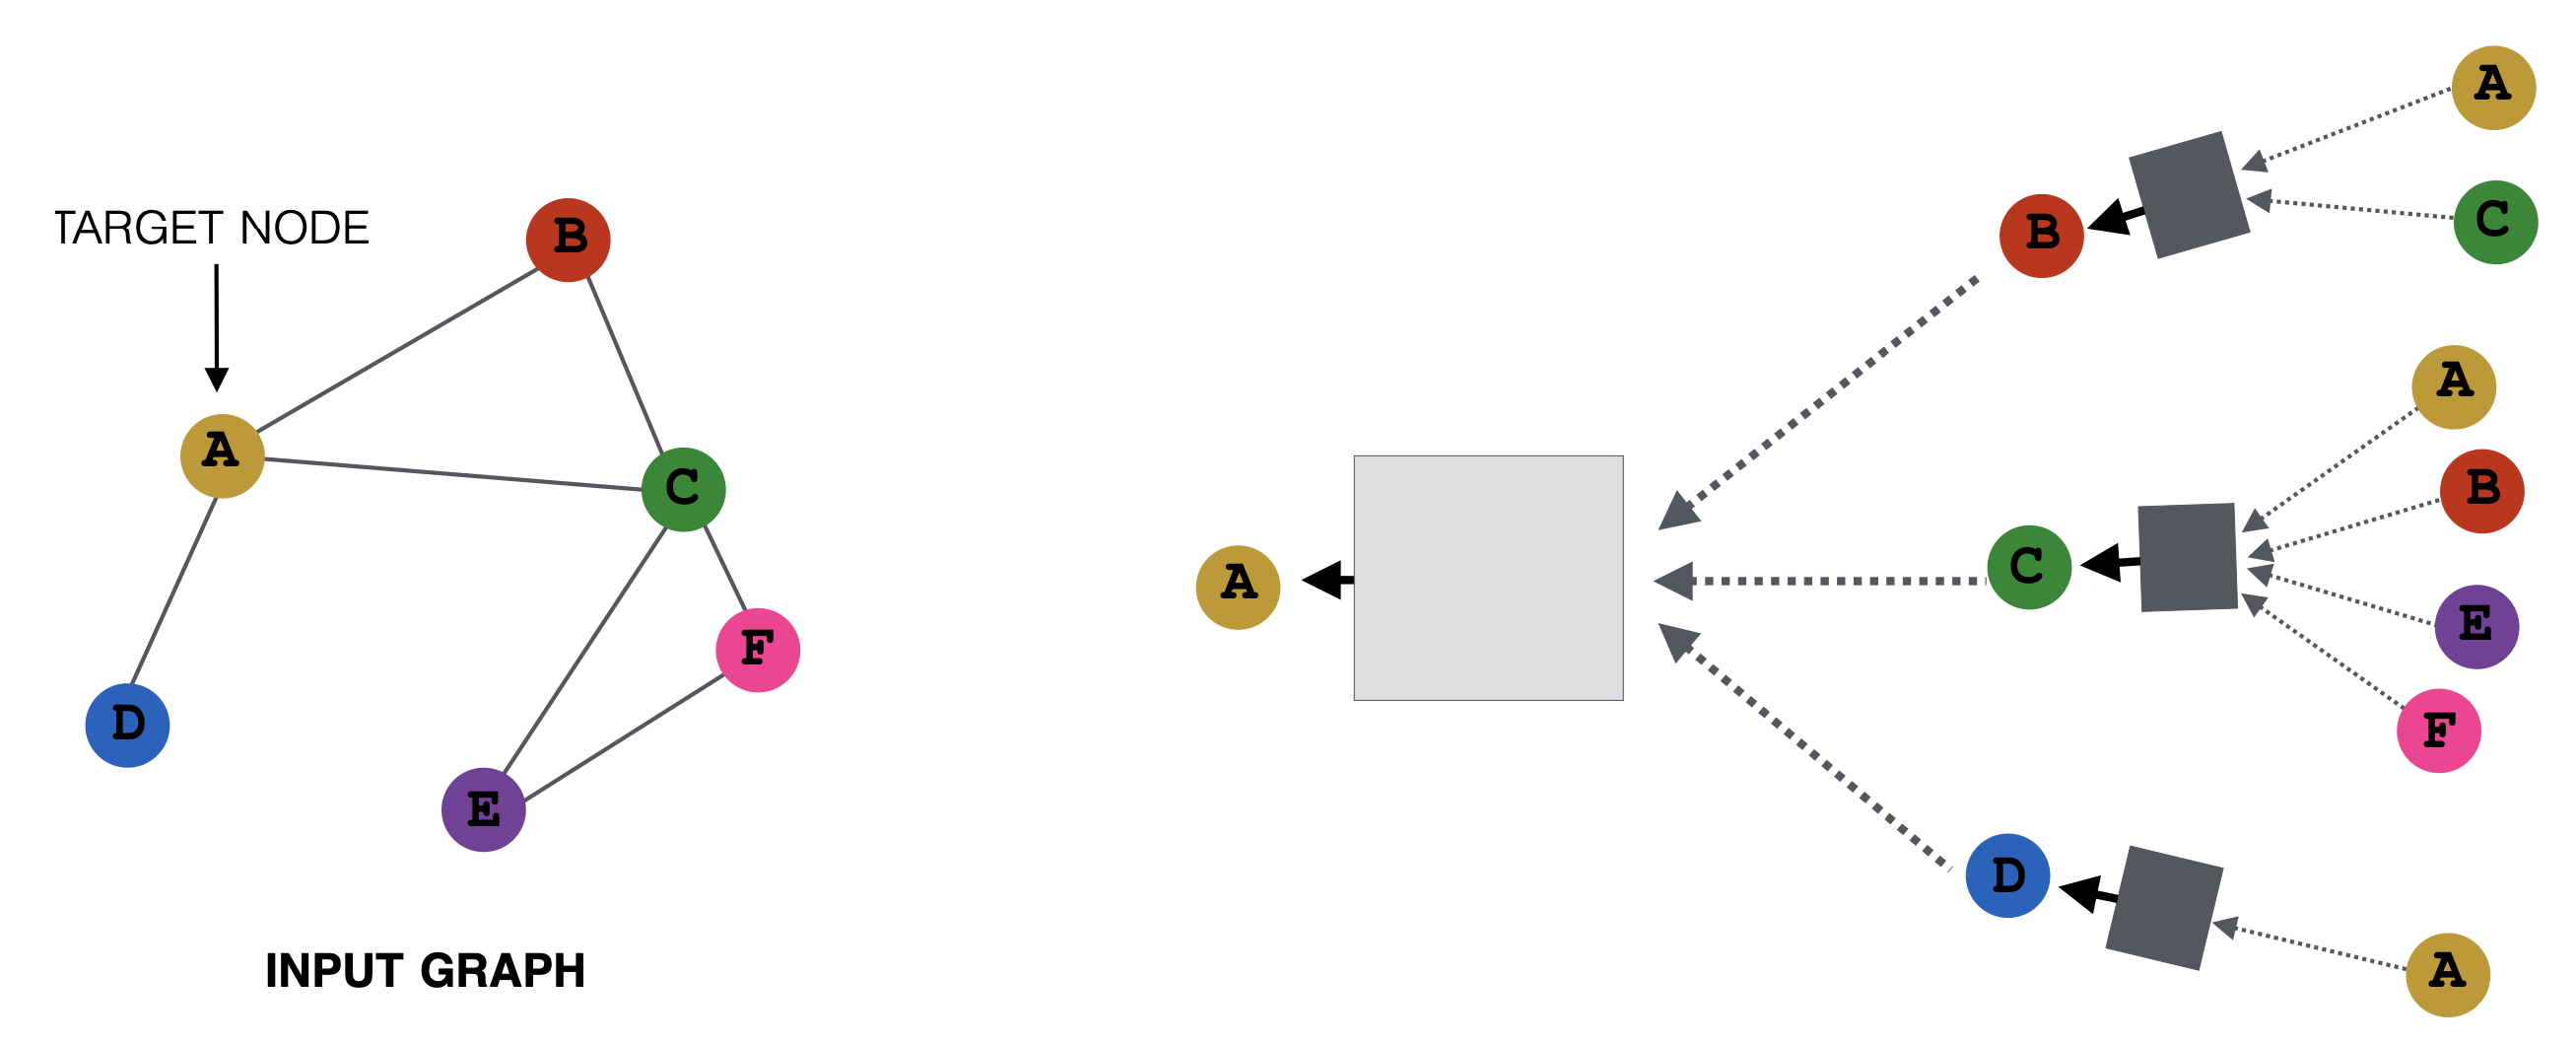
\includegraphics[width=0.5\textwidth]{images/graphfriends.png}
    \end{center}
    
    Our intuition here is that each node define a unique computational graph. 
    
       \begin{center}
        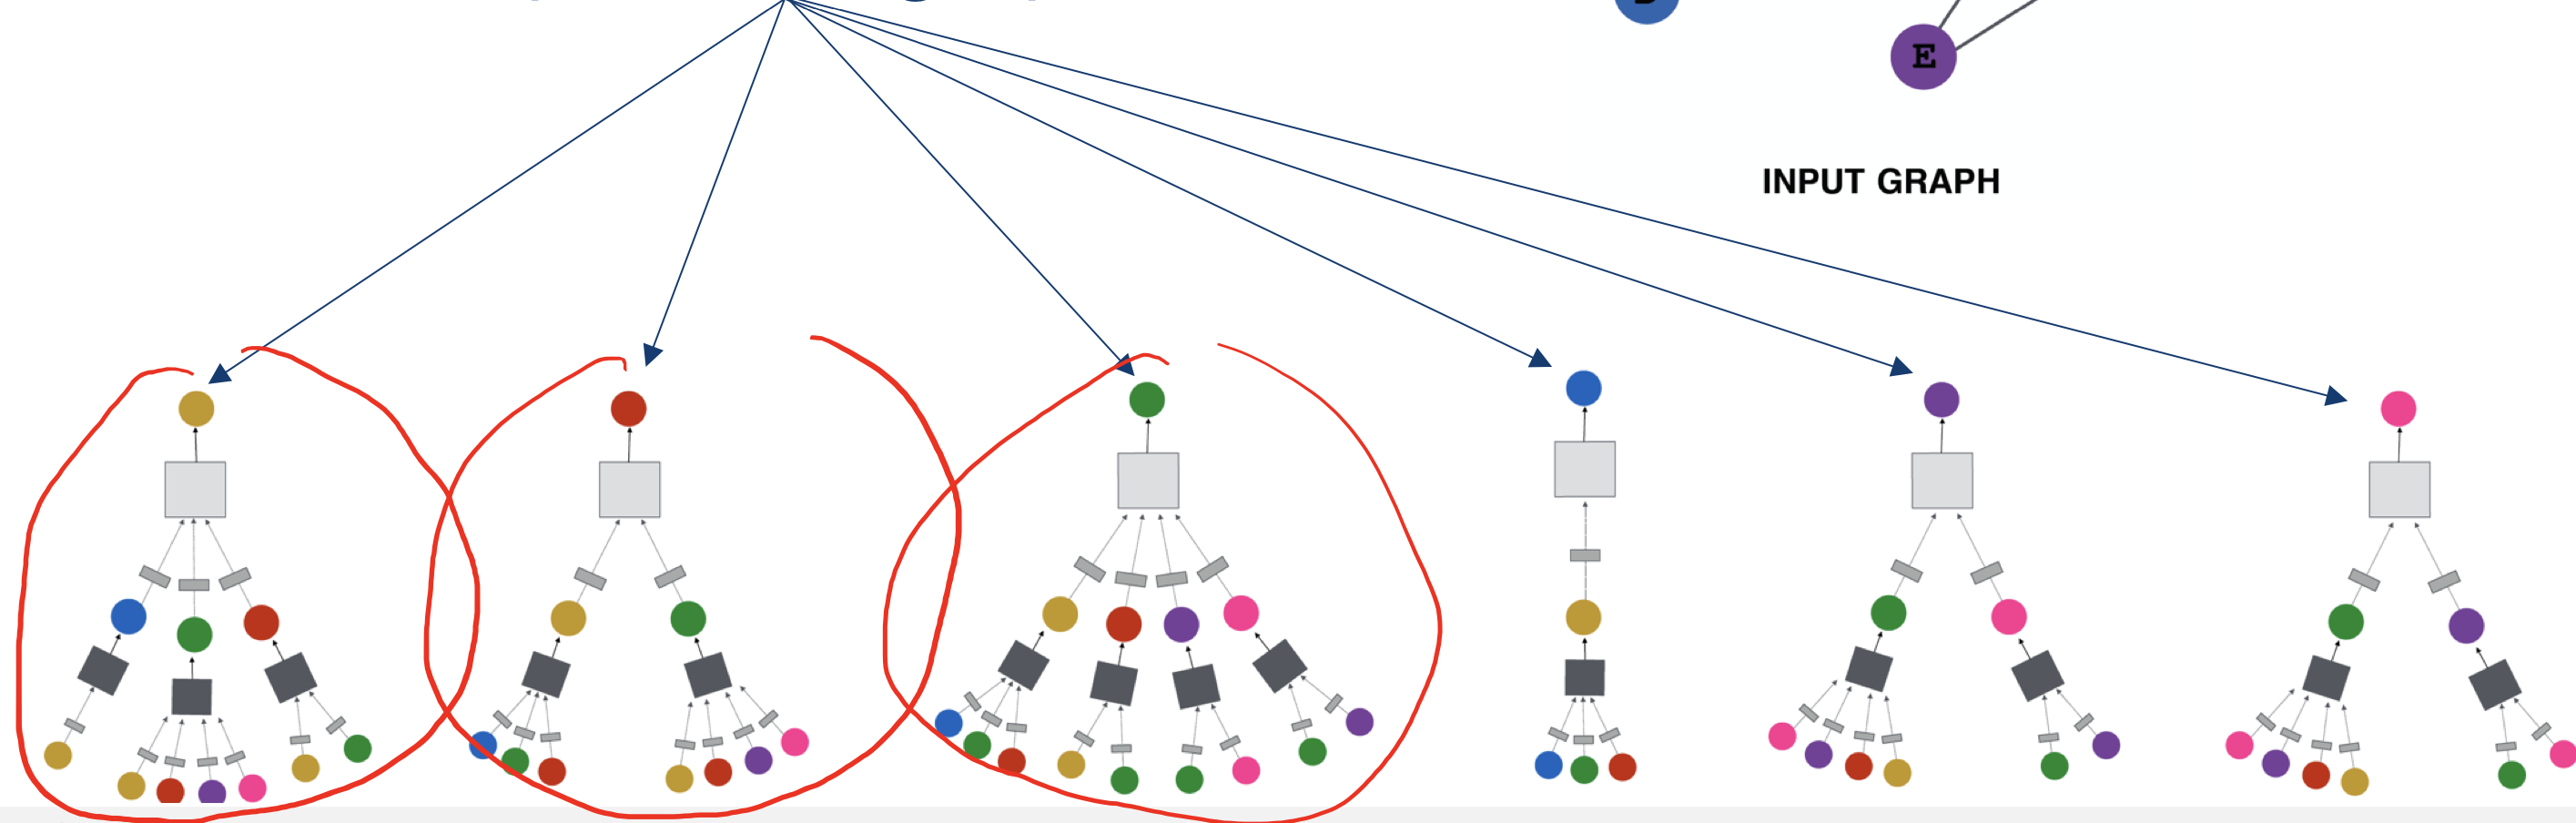
\includegraphics[width=0.5\textwidth]{images/compgraph.png}
    \end{center}
    
    This means that nodes have embeddings at each layer, and the model can be arbitrarily big. 
    
    The essence of this approach is that from one node, we can create a set of neighbours. Hence this node has ´´aggregated'' its neighbors. 
    
    This means that layer-0 has embedding of node $u$ in its input feature vector $x_u$. 
    
    A key distinction is in how different approaches aggregate information across the layers. A basic approach is to average neighbor information and apply a neural network. 
    
           \begin{center}
        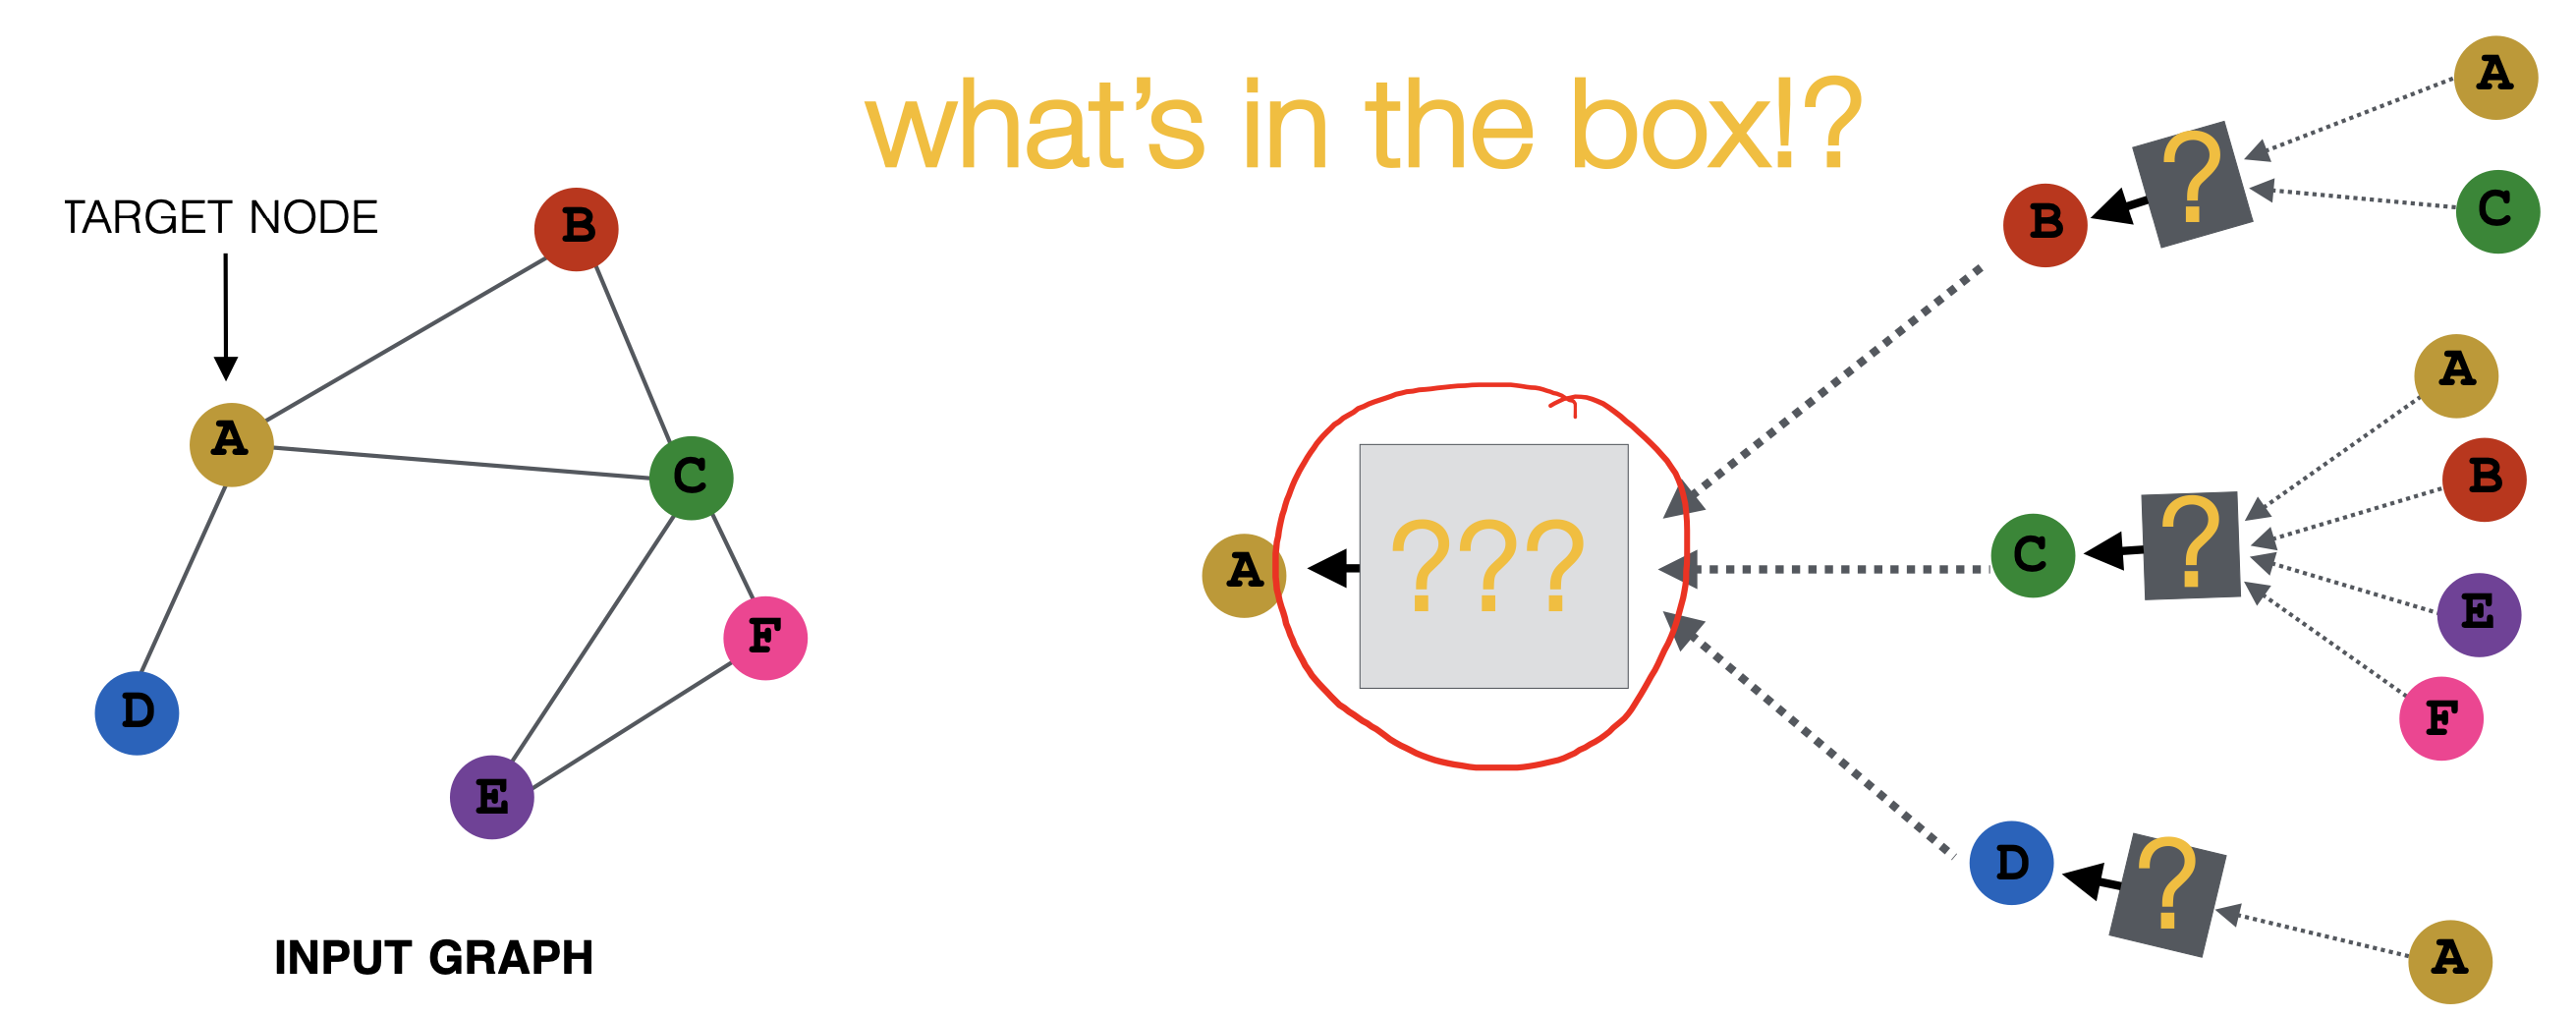
\includegraphics[width=0.5\textwidth]{images/whatsinthebox.png}
    \end{center}
    
    We start with the initial layer $0$ embeddings that are equal to node features $h_v^0 = x_v$. The $k$th layer embedding of $v$ is defined as \m{
        h_v^k = \sigma (W_k \sum_{u \in N(v)} \frac{h_u^{k-1}}{|N(v)|} + B_k h_v^{k-1}), \forall k > 0
    }
    $\sigma$ is a non-linear function such as ReLU or tanh. The sum is the average of neighbour's previous layers embeddings. 
    
    We need to define a loss function that can optimize our embeddings. $W$ and $B$ are the trainable matrices that contain what we learn. After $k$-layers of neighborhood aggregation, we get output embeddings for each node. We can feed these embeddings into any loss function and run SGD to train the aggregation parameters. 
    
    We can also rewrite our model
    \m{
        H^{l+1} = \sigma(H^l W^l + \tilde{A}H^l W_1^l)
    }
    Where $\tilde{A} = D^{-\frac{1}{2}}AD^{-\frac{1}{2}}$. We can use a supervised loss function based on things such as random walks, graph factorization or other models so that we have similar embeddings. We can also share parameters in the encoder, which allows for inductive learning. \footnote{elaborate inductive learning}
    
\subsubsection{Graph convolutions networks}
    A slight variation on the neighborhood aggregation idea is 
    \m{
        h_v^k = \sigma(W_k \sum_{u \in N(v) \cup u} \frac{h_u^{k-1}}{\sqrt{|Nu)| |N(v)|}})
    }
    So if a neighborhood has a lot of connections, it should be less important. We use the same matrix for self and neighbour embeddings, the different is that we use per-neighbor normalization.
    
    It has been found emperically to give better results. It results in more parameter sharing, and down-weights high-degree neighbbours. 
    
    We can efficiently implement it using sparse batch operations
    \m{
        H^{k+1} = \sigma(D^{-\frac{1}{2}} \tilde{A}D^{-\frac{1}{2}}H^k W_k)
    }
    Where $\tilde{A} = A + I$. (DAD in the equation is called the Laplacian matrix operator). Note that $D$ is the diagonal degree matrix. Here we have $O(|E|)$ time complexity overall. 
    

\subsubsection{GraphSAGE}
    So far we have aggregated the neighbor messages by taking their weighted average, but we can do better. We could for example use any differentiable function that maps set of vectors to a single vector. So, if we use a generalized aggregation we get \m{
        h_v^k = \sigma([W_k \cdot AGG(\set{h_u^{k-1}, \forall u \in N(v)}), B_k h_v^{k-1}])
    }
    
    Here we concatenate self embedding of neighbor embedding. We also use a generalized aggregation. Some variants are
    \begin{itemize}
        \item \textbf{Mean:} Take weighted average of neighbours \m{
            AGG = \sum_{u \in N(v)} \frac{h_u^{k-1}}{|N(v)|}
        }
        \item \textbf{Pool:} Transform neighbor vectors and apply symmetric vector function \m{
            AGG = \gamma (\set{Q h_u^{k-1}, \forall u \in N(v)})
        }
        Where we take element-wise mean/max
    \item \textbf{LSTM:} Apply LSTM to reshuffled neighbors \m{
        AGG = LSTM([h_u^{k-1}, \forall u \in \pi(N(v))])
    }
    \end{itemize}